\documentclass[authorontitle=true]{bfhbeamer}
\usepackage{amsmath}
\usepackage{pgfpages}
\usepackage{listings}
\usepackage{color}
\definecolor{lightgray}{rgb}{.9,.9,.9}
\definecolor{darkgray}{rgb}{.4,.4,.4}
\definecolor{purple}{rgb}{0.65, 0.12, 0.82}

\lstdefinelanguage{JavaScript}{
    keywords={break, case, catch, continue, debugger, default, delete, do, else, false, finally, for, function, if, in, instanceof, new, null, return, switch, this, throw, true, try, typeof, var, void, while, with},
    morecomment=[l]{//},
    morecomment=[s]{/*}{*/},
    morestring=[b]',
    morestring=[b]",
    ndkeywords={class, export, boolean, throw, implements, import, this},
    keywordstyle=\color{blue}\bfseries,
    ndkeywordstyle=\color{darkgray}\bfseries,
    identifierstyle=\color{black},
    commentstyle=\color{purple}\ttfamily,
    stringstyle=\color{red}\ttfamily,
    sensitive=true
}

\lstset{
    language=JavaScript,
    backgroundcolor=\color{lightgray},
    extendedchars=true,
    basicstyle=\footnotesize\ttfamily,
    showstringspaces=true,
    showspaces=true,
    tabsize=2,
    breaklines=true,
    showtabs=false,
    captionpos=b
}

\setbeamertemplate{page number in head/foot}[framenumber]
\title{Decibel Threshold Event Displayer}
\subtitle{BTI3031 Project 1 | Final Presentation}
\author{Dominic Gernert, Lukas von Allmen, Darius Degel}

% macro which adds fancy ToC to all sections
\AtBeginSection[]
{
  \begin{frame}
    \frametitle{Table of Contents}
    \begin{columns}
      \column{0.6\textwidth}
        \tableofcontents[
            sectionstyle=show/shaded,
            subsectionstyle=show/show/hide
        ]
      \column{0.4\textwidth}
          
\includegraphics[width=0.6\textwidth]{../assets/ear.png}
    \end{columns}
  \end{frame}
}

\begin{document}
%\pgfpagesuselayout{2 on 1}[a4paper, border shrink=5mm]
\maketitle
\section{Problem Description}\label{sec:problem-description}
% ---------------------------------------------------------------------------
% Initial Situation
\begin{frame}
    \frametitle{Initial Situation}
    \centering
    \includegraphics[width=0.8\linewidth]{../assets/collage_sound_pollution.png}
\end{frame}
% ---------------------------------------------------------------------------

% ---------------------------------------------------------------------------
% Project Goals
\begin{frame}
    \frametitle{Project Goals}
    \begin{itemize}[<+->]
        \large
        \item Analyze Audio File
        \item Summarize findings in a PDF
        \item Easy to use
    \end{itemize}
\end{frame}
% ---------------------------------------------------------------------------

% Audio Files
\begin{frame}
    \frametitle{Audio Files}
    \centering
    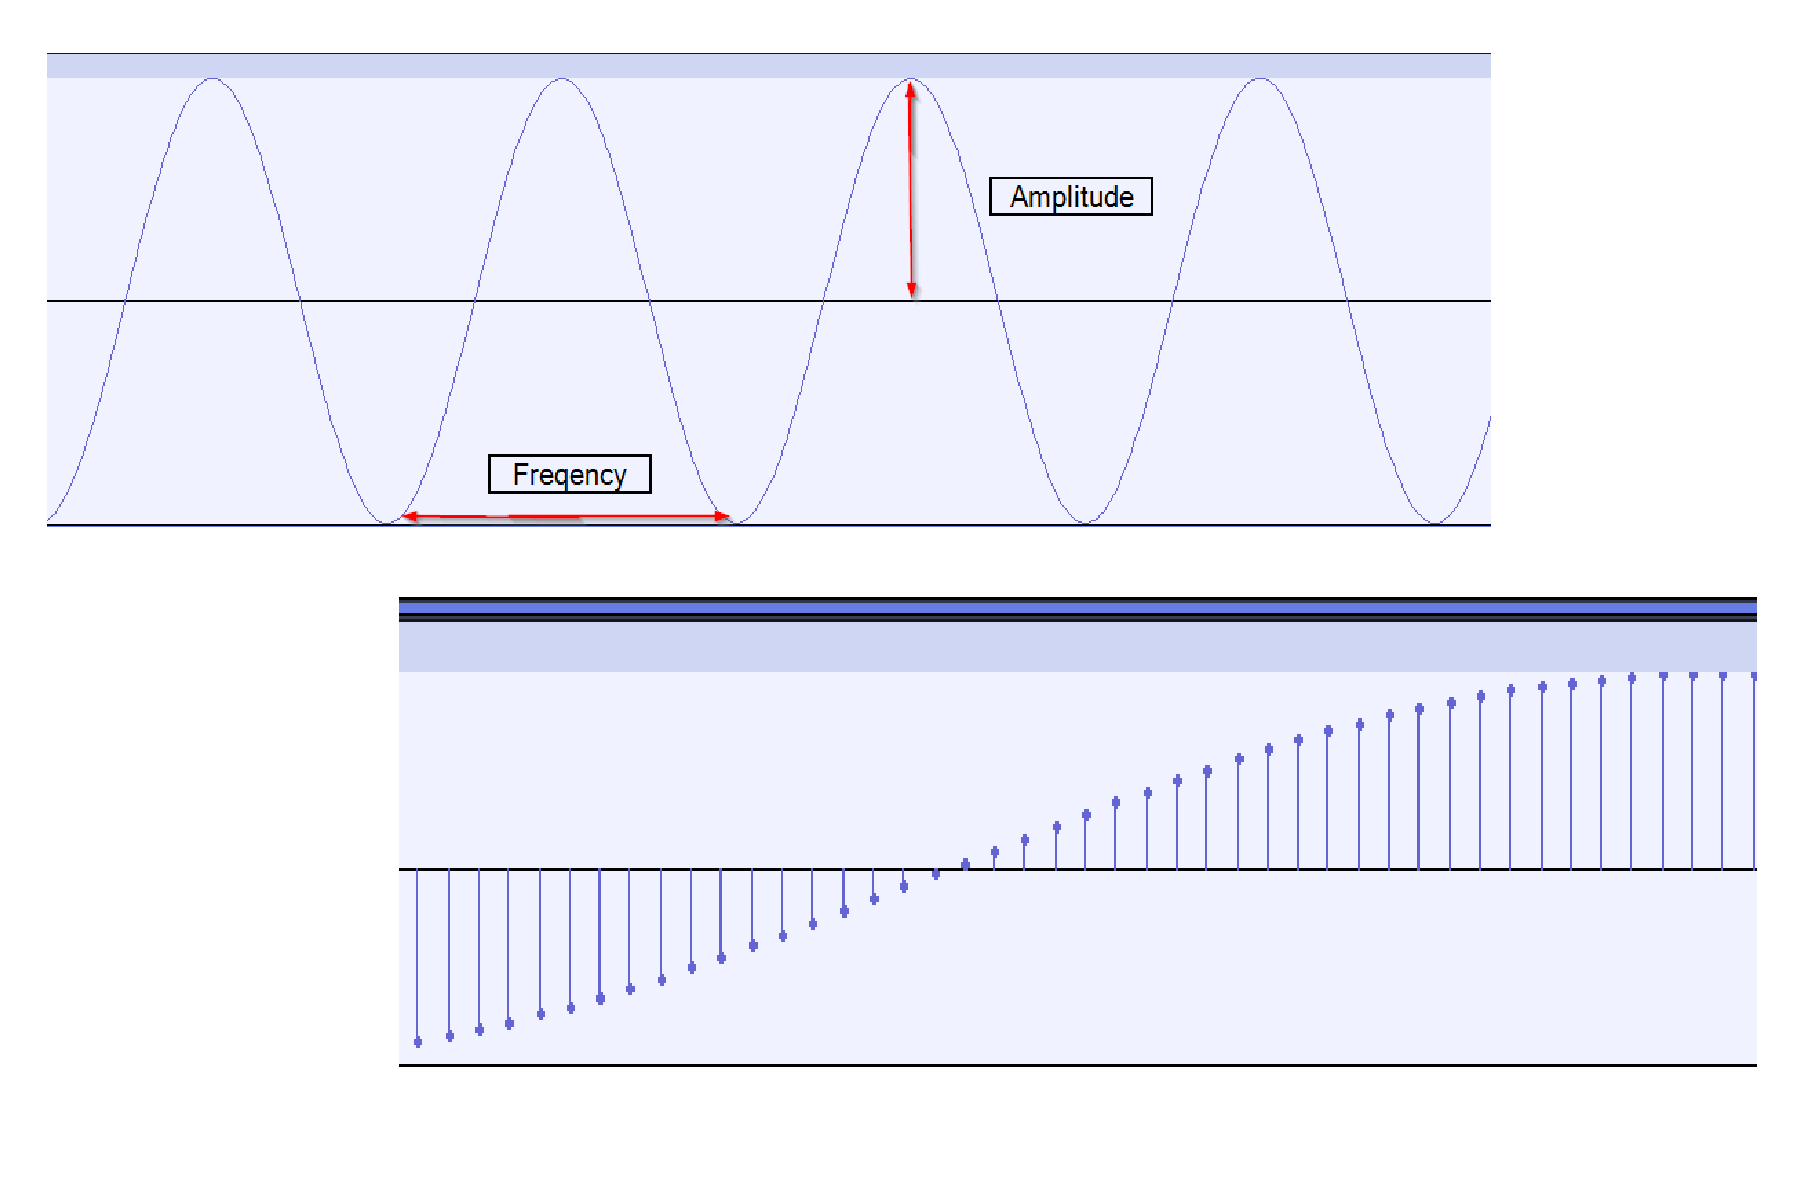
\includegraphics[width=0.8\linewidth]{../assets/audiofile_description.png}
\end{frame}
% ---------------------------------------------------------------------------

% Measuring the Sound Level
\begin{frame}
    \frametitle{Measuring the Sound Level}
    \centering
    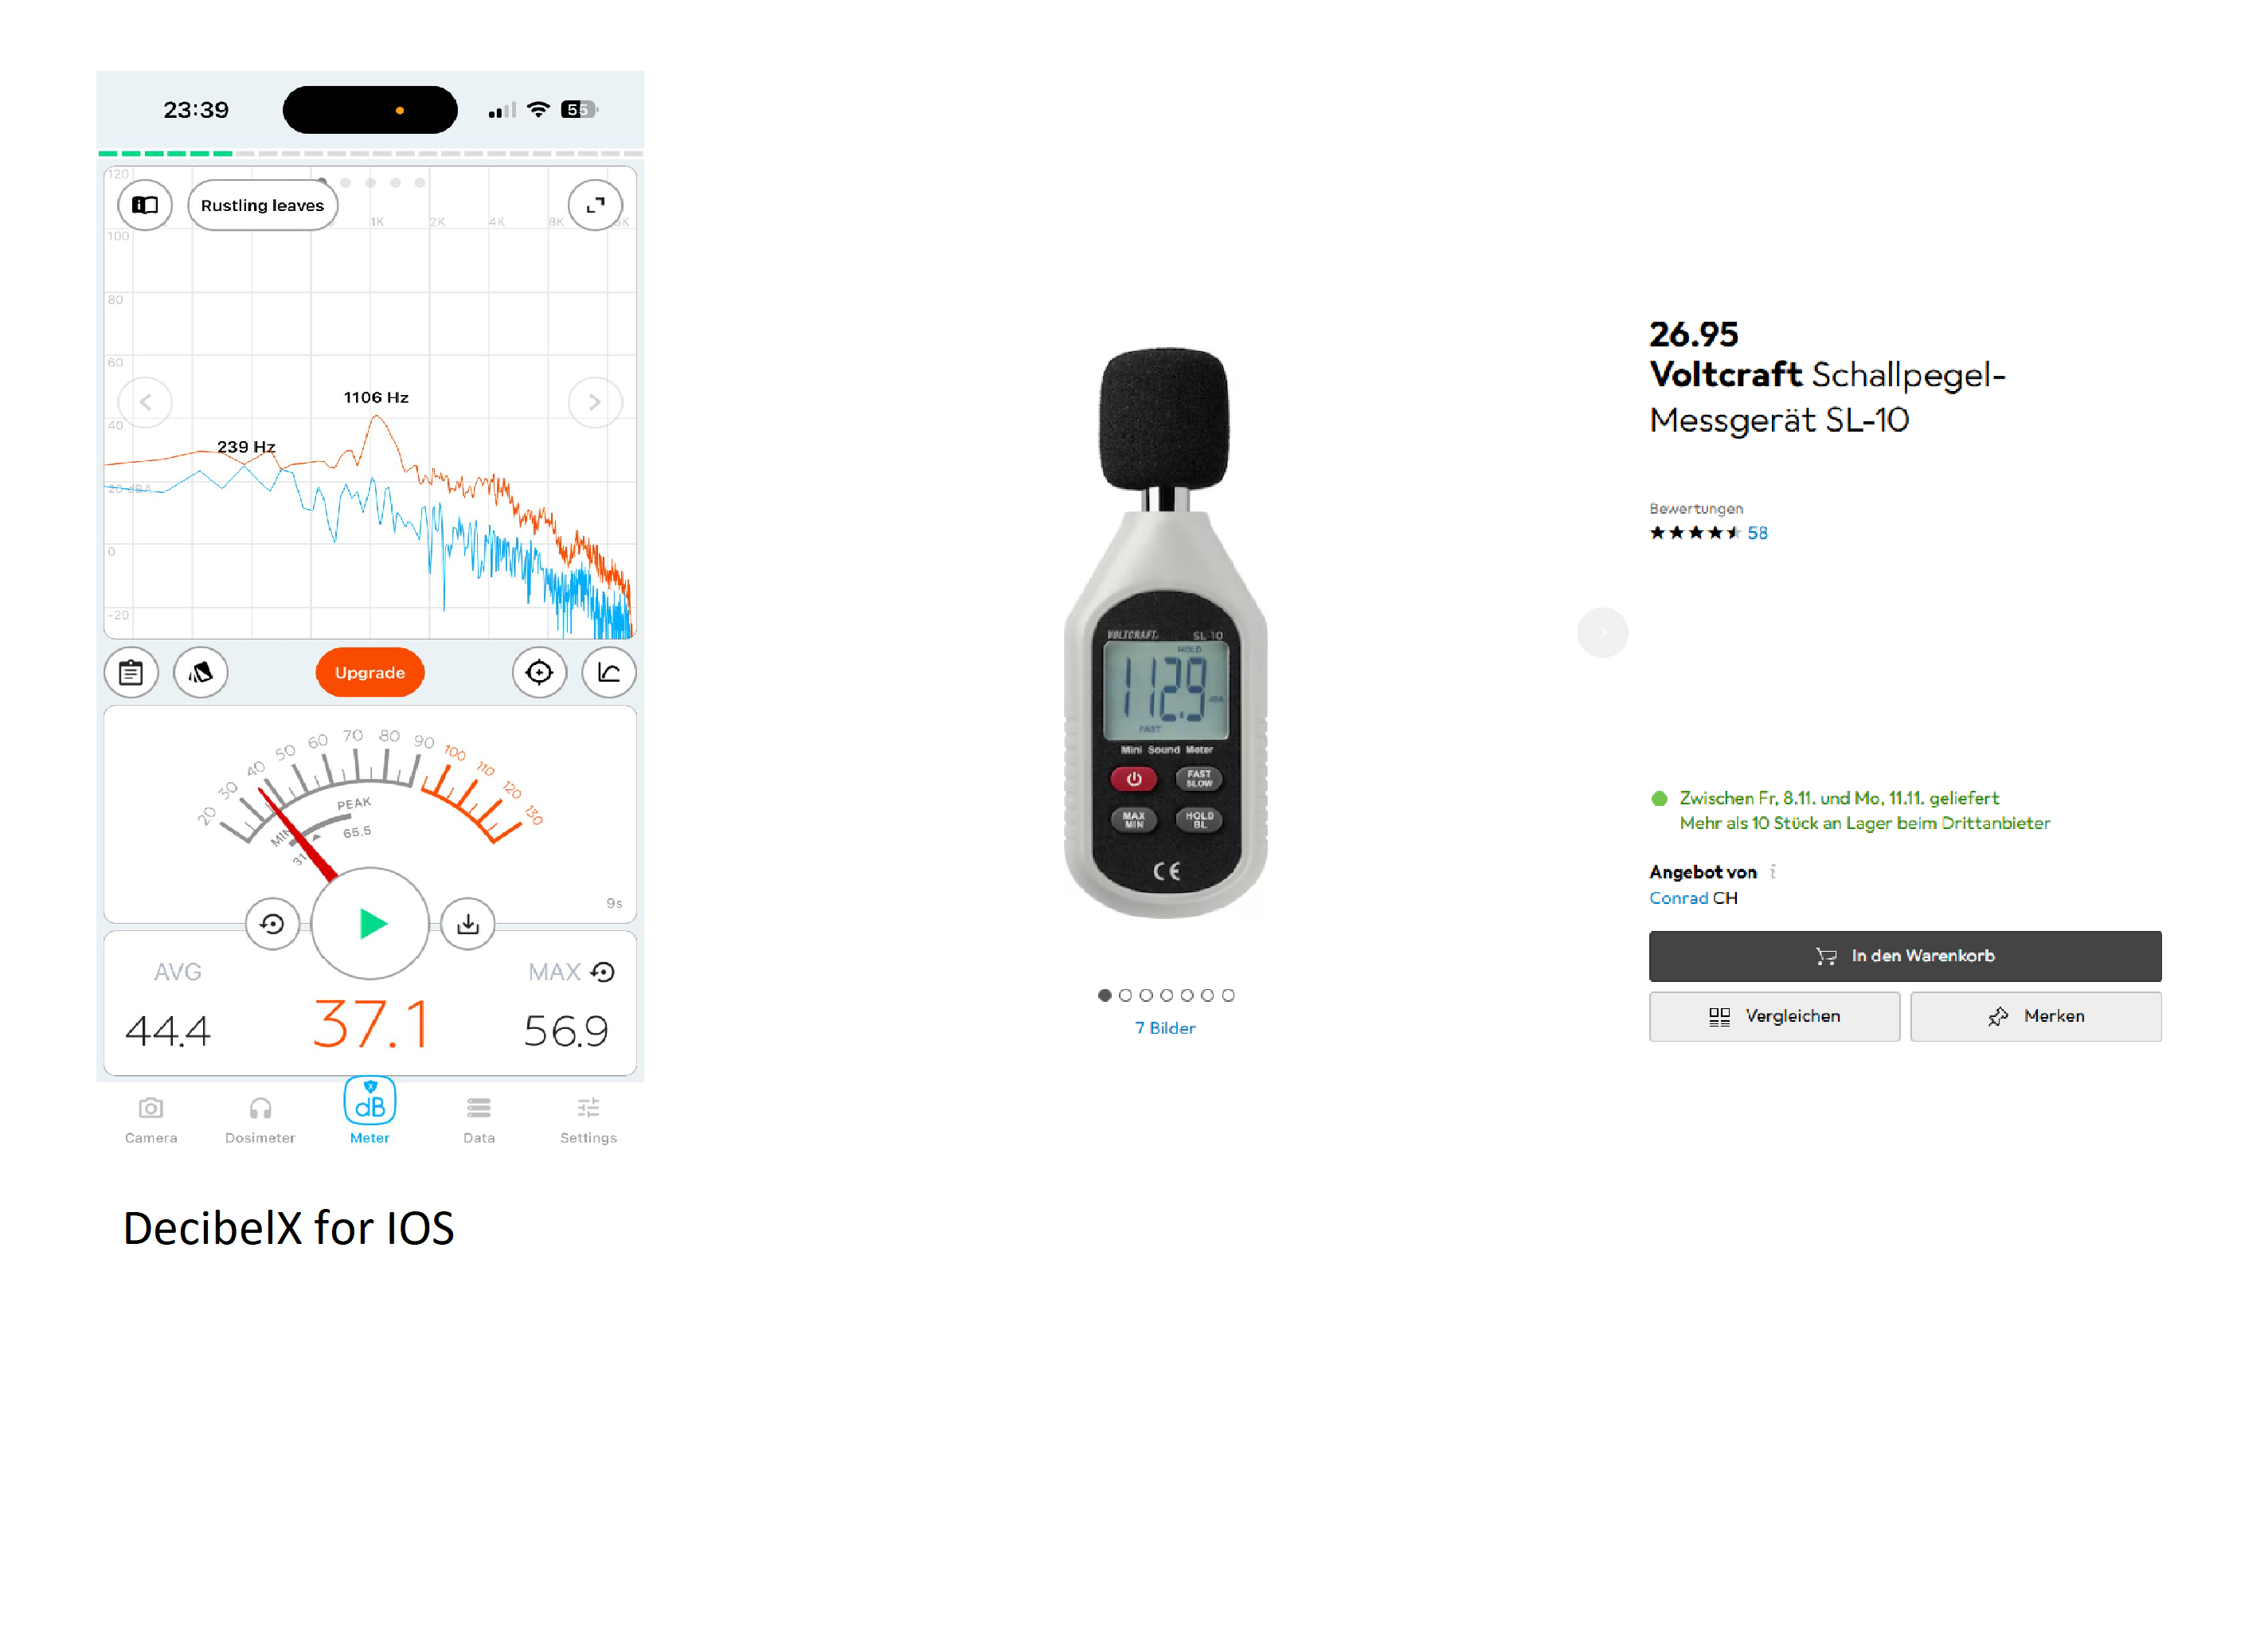
\includegraphics[width=0.8\linewidth]{../assets/measure_sound_level.png}
\end{frame}
% ---------------------------------------------------------------------------

% Requirements
\begin{frame}
    \frametitle{Requirements}
    \begin{itemize}[<+->]
        \large
        \item Take .wav file, threshold and additional reference values as input
        \item Analyze and Summarize 
        \begin{itemize}
            \large
            \item Metadata
            \item Plot
        \end{itemize}
        \item User should not need any Technical know-How
        \item Platform independent
        \item Multiple Languages
    \end{itemize}
\end{frame}
% ---------------------------------------------------------------------------
\section{Implementation}\label{sec:implementation}
\section{Implementation}
Lorem ipsum

\subsection{Architecture}
Lorem ipsum

\subsection{Processes}
Lorem ipsum


\section{Scrum}\label{sec:scrum}
% ---------------------------------------------------------------------------
% Scrum Roles
\begin{frame}
    \frametitle{Scrum Roles}
    \begin{columns}
        % Dr. Simon Kramer
        \column{0.25\textwidth}
        \centering
        
\includegraphics[width=0.45\linewidth]{../assets/avatar_placeholder.jpg} \\
        \textbf{Dr. Simon Kramer} \\ \small{Tutor \& Stakeholder} \par\vspace{0.5cm}
        % Dominic Gernert
        \column{0.25\textwidth}
        \centering
        
\includegraphics[width=0.45\linewidth]{../assets/avatar_placeholder.jpg} \\
        \textbf{Dominic Gernert} \\ \small{Product Owner} \par\vspace{0.5cm}
    \end{columns}
    \begin{columns}
        % Lukas von Allmen
        \column{0.25\textwidth}
        \centering
        
\includegraphics[width=0.45\linewidth]{../assets/avatar_placeholder.jpg} \\
        \textbf{Lukas von Allmen} \\ \small{Scrum Master}
        % Darius Degel
        \column{0.25\textwidth}
        \centering
        
\includegraphics[width=0.45\linewidth]{../assets/avatar_placeholder.jpg} \\
        \textbf{Darius Degel} \\ \small{Developer}
\end{columns}
\end{frame}
% ---------------------------------------------------------------------------

% ---------------------------------------------------------------------------
% Backlog
\begin{frame}
    \frametitle{Backlog}
    \begin{columns}
        \column{0.5\textwidth}
        \begin{itemize}
            \large
            \item Epics \ensuremath{\approx} Milestones
            \item Impediments
            \item Development Board
        \end{itemize}
        \column{0.5\textwidth}
        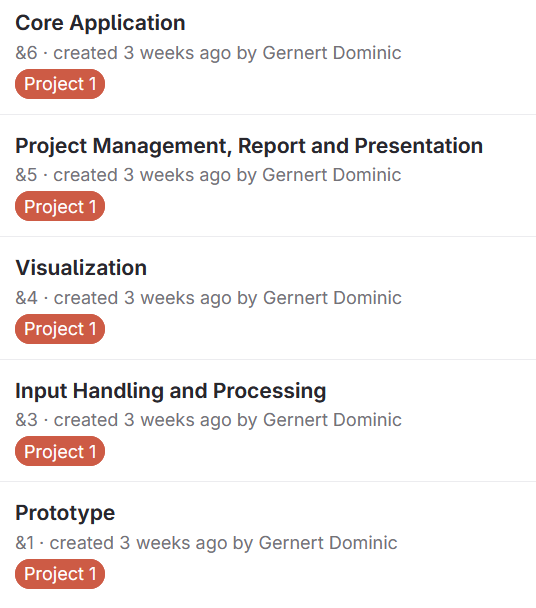
\includegraphics[width=0.8\linewidth]{../assets/epics_interim_presentation.png}
    \end{columns}
\end{frame}
% ---------------------------------------------------------------------------

% ---------------------------------------------------------------------------
% Backlog cont.
\begin{frame}
    \frametitle{Backlog}
    \centering
    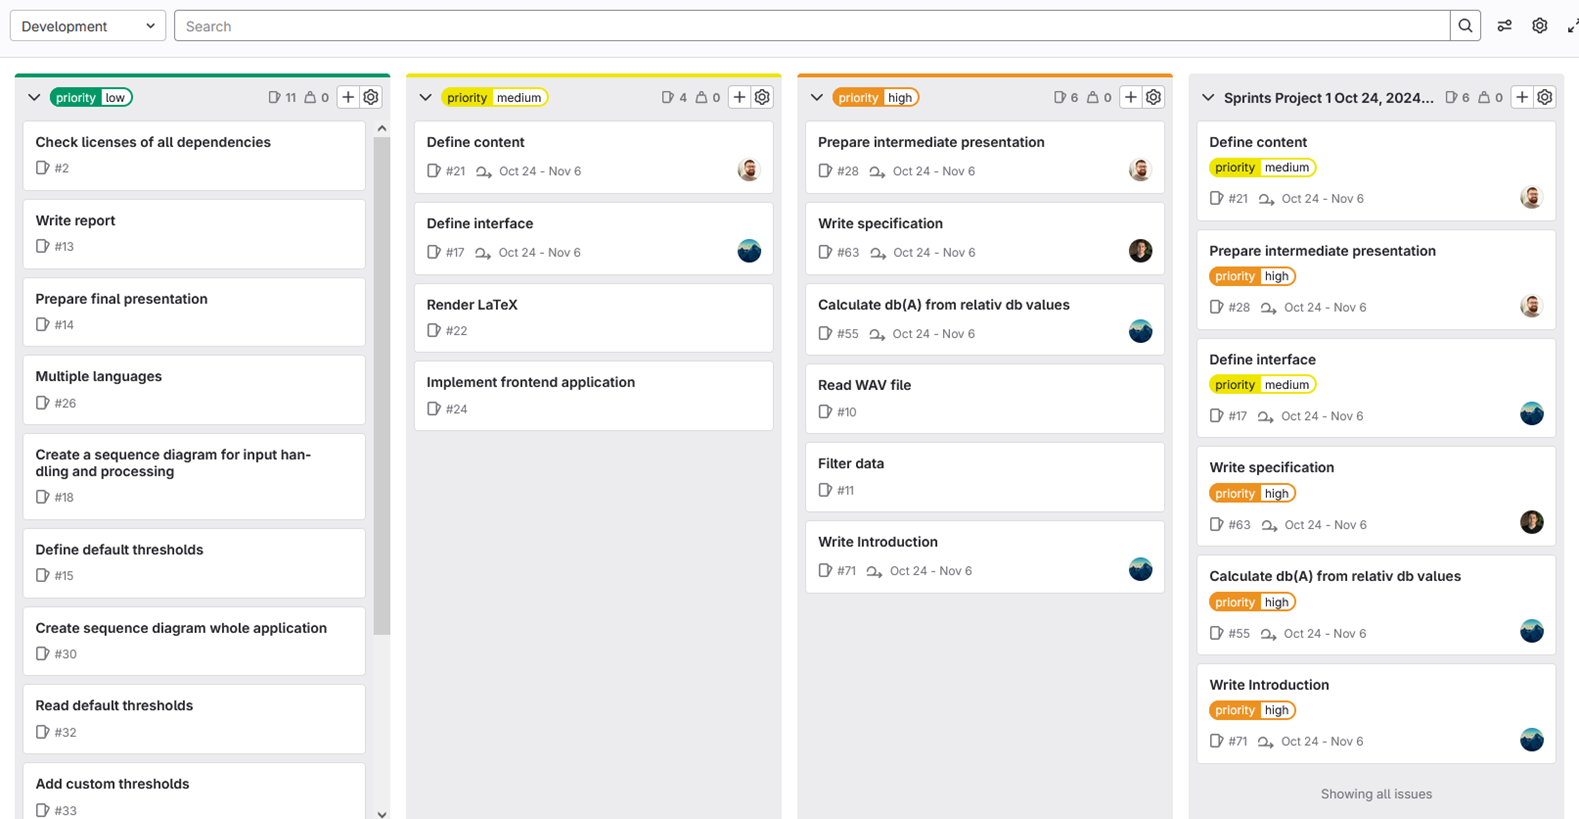
\includegraphics[width=0.85\linewidth]{../assets/backlog_interim_presentation.png}
\end{frame}
% ---------------------------------------------------------------------------

% ---------------------------------------------------------------------------
% Sprint Goals
\begin{frame}
    \frametitle{Sprint Goals}
    \begin{itemize}
        \large
        \item S.M.A.R.T
        \item Product Focus
    \end{itemize}
    \par\vspace{0.5cm}
    \begin{example}
        Prototypes with two different technologies are implemented and their pros and cons are evaluated.
    \end{example}
\end{frame}
% ---------------------------------------------------------------------------

% ---------------------------------------------------------------------------
% Review & Retro
\begin{frame}
    \frametitle{Review \& Retro}
    \centering
    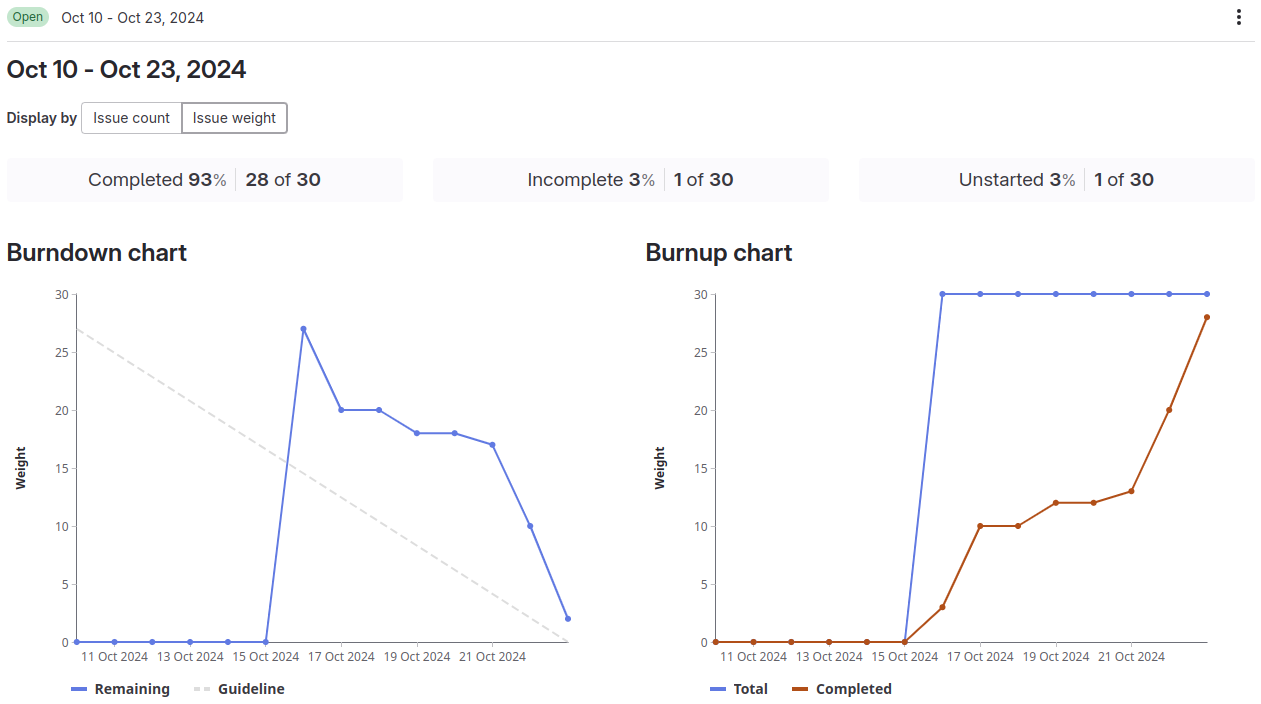
\includegraphics[width=0.84\linewidth]{../assets/burndown_sprint_001.png}
\end{frame}
% ---------------------------------------------------------------------------

% ---------------------------------------------------------------------------
% Review & Retro cont.
\begin{frame}
    \frametitle{Review \& Retro}
    \begin{columns}
    \column{0.5\textwidth}
    \large
    \textbf{Review}
    \begin{itemize}
        \large
        \item Demo
        \item Done / Not Done
        \item Goal Attainment
    \end{itemize}
    \column{0.5\textwidth}
    \large
    \textbf{Retro}
    \begin{itemize}
        \large
        \item What went well?
        \item What problems did we encounter?
        \item What are we improving in the future?
    \end{itemize}
    \end{columns}
\end{frame}
% ---------------------------------------------------------------------------

% ---------------------------------------------------------------------------
% Adaptations
\begin{frame}
    \frametitle{Adaptations}
    \begin{itemize}
        \large
        \item Product Owner
        \item No Release Plan
        \item Retro
        \begin{itemize}
            \large
            \item Shorter first Retro
            \item Successes, Problems, Improvements 
        \end{itemize}
    \end{itemize}
\end{frame}
% ---------------------------------------------------------------------------
\section{Demo}\label{sec:demo}
\begin{frame}
    \frametitle{TEST}
\end{frame}
\section{Conclusion \& Future Work}\label{sec:conclusion}
\begin{frame}
    \frametitle{Conclusion}
\end{frame}
\end{document}